%        File: COMP3121Ass1.tex
%     Created: Sun Mar 20 06:00 PM 2016 A
% Last Change: Sun Mar 20 06:00 PM 2016 A
%
\documentclass[11pt, a4paper]{article}
\usepackage{listings}
\usepackage[margin=0.8in]{geometry}
\usepackage{amsmath}
\usepackage{graphicx}
\usepackage{fancyhdr}
\pagestyle{fancy}
\title{COMP3121 Assignment 2}
\author{Alex Nguyen z3379933}
\date{09/04/16}
\lhead{Alex Nguyen z3379933}

\begin{document}

\maketitle{\textbf{Question 1a)}}
The Fibonacci function $F(n)$ can be summarised below:


\[ F(n) = \left\{ \begin{array}{ll}
         0 & \mbox{if $n = 1$};\\
         1 & \mbox{if $n =  2$};\\
        F(n-1) + F(n-2) & \mbox{if $n \ge 2$}.\end{array} \right. \] 

Required to show:
      \begin{equation}
        \begin{pmatrix}
          F(n+1) & F(n) \\
          F(n) & F(n-1)
        \end{pmatrix} 
        =
        \begin{pmatrix}
          1 & 1 \\
          1 & 0
        \end{pmatrix} ^n
      \end{equation}

Taking element of RHS: ( where n = 2)
\[ \begin{pmatrix}
          1 & 1 \\
          1 & 0
        \end{pmatrix} 
        \begin{pmatrix}
          1 & 1 \\
          1 & 0
        \end{pmatrix} =
        \begin{pmatrix}
          2 & 1 \\
          1 & 0
        \end{pmatrix} =
        \begin{pmatrix}
          F(2) + F(1) & F(1) + F(0) \\
          F(1) + F(0) & F(0) 
      \end{pmatrix} \]
        \[ \begin{pmatrix}
            F(3) & F(2) \\
            F(2) & F(1)
        \end{pmatrix} =
        \begin{pmatrix}
            1 & 1 \\
            1 & 0
        \end{pmatrix} ^2
      \]
 Now, when n = 3:
\[ \begin{pmatrix}
          1 & 1 \\
          1 & 0
        \end{pmatrix}^2 
        \begin{pmatrix}
          1 & 1 \\
          1 & 0
        \end{pmatrix} =
        \begin{pmatrix}
          2 + 1 & 2 + 0 \\
          1 + 1 & 1 + 0
        \end{pmatrix} =
        \begin{pmatrix}
          F(3) + F(2) & F(2) + F(1) \\
          F(2) + F(1) & F(1) + F(0) 
      \end{pmatrix} \]
        \[ \begin{pmatrix}
            F(4) & F(3) \\
            F(3) & F(2)
        \end{pmatrix} =
        \begin{pmatrix}
            1 & 1 \\
            1 & 0
        \end{pmatrix} ^3
      \]
 Extend for n'th term:
\[ \begin{pmatrix}
          1 & 1 \\
          1 & 0
        \end{pmatrix}^{n-1}
        \begin{pmatrix}
          1 & 1 \\
          1 & 0
        \end{pmatrix} =
        \begin{pmatrix}
          F(n) + F(n-1) & F(n-1) + F(n-2) \\
          F(n-1) + F(n-2) & F(n-2) + F(n-3) 
      \end{pmatrix} \]
      But remembering \[ F(n) = F(n-1) + F(n-2); n \ge 2: \]
      The above becomes:
        \[ \begin{pmatrix}
            F(n+1) & F(n) \\
            F(n) & F(n-1)
        \end{pmatrix} 
      \]

      Thus, equation (1) is true.


      \maketitle{\textbf{Question 1b)}

From part a), equation (1):
        \[\begin{pmatrix}
          F(n+1) & F(n) \\
          F(n) & F(n-1)
        \end{pmatrix} 
        =
        \begin{pmatrix}
          1 & 1 \\
          1 & 0
      \end{pmatrix} ^n \]

Take RHS. This is the original matrix multiplied by itself n times:
        \[\begin{pmatrix}
          1 & 1 \\
          1 & 0
        \end{pmatrix} ^n =
        \bigg\{ \begin{pmatrix}
          1 & 1 \\
          1 & 0
        \end{pmatrix}
        \begin{pmatrix}
          1 & 1 \\
          1 & 0
        \end{pmatrix}
        \dots
        \begin{pmatrix}
          1 & 1 \\
          1 & 0
      \end{pmatrix} \bigg\} \mbox{n multiplications}\]

Minimise multiplication steps by dividing into groups of the original matrix squared:
        \[\begin{pmatrix}
          1 & 1 \\
          1 & 0
        \end{pmatrix} ^n =
        \bigg\{ \begin{pmatrix}
          1 & 1 \\
          1 & 0
        \end{pmatrix}
        \begin{pmatrix}
          1 & 1 \\
          1 & 0
        \end{pmatrix}\bigg\}
        \dots
        \bigg\{ \begin{pmatrix}
          1 & 1 \\
          1 & 0
      \end{pmatrix}
        \begin{pmatrix}
          1 & 1 \\
          1 & 0
      \end{pmatrix} \bigg\} =
      \bigg\{ \begin{pmatrix}
          1 & 1 \\
          1 & 0
        \end{pmatrix} ^2 \bigg\}
        \dots
        \bigg\{ \begin{pmatrix}
          1 & 1 \\
          1 & 0
      \end{pmatrix} \bigg\}^2
    \mbox{$n/2$ groups}\]
 This essentially performs the multiplications by raising by powers of two. As Each group will
 have the same result matrix at each step (squares at each stage), the steps taken to get to the
 n'th final matrix depends on the number of power. This progresses clearly in $log_2 n$
 steps - $n/2$ groups of squareds, then $n/4$ groups of powers to the 4th.
This works exactly for n even (even powers)

In the n odd scenario, perform the same method to the nearest even number lower than n and multiply by
        $ \begin{pmatrix}
          1 & 1 \\
          1 & 0
      \end{pmatrix} $ to obtain the matrix relevant to the final power. This gives $log_2n + 1$ steps overall.

However, from equation (1), each matrix provides the Fibonacci function for the next n. Thus,
only n-1 multiplications are needed.
        \[\begin{pmatrix}
          1 & 1 \\
          1 & 0
        \end{pmatrix} ^n =
         \begin{pmatrix}
          1 & 1 \\
          1 & 0
        \end{pmatrix}
        \begin{pmatrix}
          1 & 1 \\
          1 & 0
      \end{pmatrix}^{n-1} =
          \begin{pmatrix}
          1 & 1 \\
          1 & 0
        \end{pmatrix}
        \begin{pmatrix}
          F(n) & F(n-1) \\
          F(n-1) & F(n-2)
      \end{pmatrix}^{n-1} =   
    \]
But $\begin{pmatrix}
          1 & 1 \\
          1 & 0
      \end{pmatrix}^{n-1}$ 
      computes in $log_2 n$ steps (from above) and provides a matrix which $F(n)$ is readable from, giving $F(n)$ in $log_2 n$ steps.

\[ \left( \begin{array}{ccc}
a & b & c \\
d & e & f \\
g & h & i \end{array} \right)\] 


\maketitle{\textbf{Question 2a)}
\begin{equation}
(a+ib)(c+id) = ac + adi + bci + bdi^2 = (ac - bd) + (ad + bc)i
\end{equation}
Now, from Karatsuba trick we have:
\[(a+b)(c+d) = ac + ad + bc + bd \]
\begin{equation}
(a+b)(c+d) -ac - bd = ad + bc
\end{equation}
Substitute $(3)$ into $(2):$

\[ (a+ib)(c+id) = (ac - bd) + \big((a+b)(c+d) - ac - bd)\big)i \]
Hence, to achieve the result in 3 multiplications calculate $a \times c$ (1), $b \times d$ (2), 
find $(a+b)$ and $(c+d)$ and finally multiply the result (3).

\maketitle{\textbf{Question 2b)}
\[ (a+ib)^2 = (a+ib)(a+ib) = a^2 + b^2i^2 + 2abi= (a^2 - b^2) + (2ab)i = (a+b)(a-b) + (ab+ab)i \]
To achieve the result in 2 multiplications (and infinite integer addition) calculate $a \times b$ (1), $ab + ab$, 
find $(a+b)$ and $(a-b)$ and finally multiply the result (2).


\maketitle{\textbf{Question 2c)}}
If it can be assumed that infinite additions are acceptable as in part a) and b):
\[(a+ib)^2(c+id)^2 = \big[(a+b)(a-b)-2abi\big]\big[(c+d)(c-d)-2cdi\big]\]
Then, multiply: $ab (1)$, add and multiply: $(a+b)(a-b) (2)$, $cd (3)$, add and multiply: $(c+d)(c-d) (4)$ and finally multiply the sum result of previous multiplications (1), (2), (3), (4):
\[ \big[(2) + (1)i\big]\big[(4) + (3)i\big]\ (5)\]
Hence, the number is evaluated in 5 multiplications.

Otherwise if the addition assumption does not hold, use value representation of complex number as a polynomial with 5 large integer multiplications and evaluate coefficients.
Set up result as $C(x)$, the multiplication of two polynomials $P(x)$ and $Q(x)$ with coefficients as large integers $A_n$ and $B_n$:
\[(a+ib)^2(c+id)^2 = P(x)\times Q(x) = C(x) \] where x = i
\[P(x) = b^2x^2 + 2abx + a^2 = A_2x^2 + A_1x + A_0\]
\[Q(x) = d^2x^2 + 2cdx + d^2 = B_2x^2 + B_1x + B_0\]
where:
\begin{align}
A_2 = b^2 ; A_1 = 2ab ; A_0 = b^2 \quad &
B_2 = d^2 ; B_1 = 2cd ; B_0 = d^2
\end{align}

Perform Evaluations at 5 points and multiply $C(x) = P(x)Q(x)$.
\begin{align}
P(-2) = A_0 - 2A_1 + 4A_2 \quad & 
Q(-2) =  B_0 - 2B_1 + 4B_2  \quad &  
C(-2) =  (A_0 - 2A_1 + 4A_2)(B_0 - 2B_1 + 4B_2)  \\  
P(-1) = A_0 - A_1 + A_2  \quad &
Q(-1) =  B_0 - B_1 + B_2  \quad & 
C(-1) =( A_0 - A_1 + A_2  )( B_0 - B_1 + B_2  )\\  
P(0) = A_0 \quad &
Q(0) = B_0 \quad &
C(0) =  A_0B_0 \\
P(1) = A_0 + A_1 + A_2  \quad &
Q(1) =  B_0 + B_1 + B_2  \quad & 
C(1) =(  A_0 + A_1 + A_2  )( B_0 + B_1 + B_2 ) \\  
P(2) = A_0 + 2A_1 + 4A_2 \quad & 
Q(2) =  B_0 + 2B_1 + 4B_2  \quad  & 
C(2) = ( A_0 + 2A_1 + 4A_2 )( B_0 + 2B_1 + 4B_2  )\\  
\end{align}


Use matrix transformation and invert to obtain vector of coefficients of C(x):
We have 5 points so the matrix will be $5\times 5$.
       \[ \begin{pmatrix}
          1 & -2 & 4 & -8 & 16 \\
          1 & -1 & 1 & -1& 1 \\
          1 & 0 & 0 & 0 & 0 \\
          1 & 1 & 1 & 1& 1 \\
          1 & 2 & 4 & 8 & 16 \\
        \end{pmatrix} 
         \begin{pmatrix}
          C_0 \\ C_1 \\ C_2 \\ C_3 \\ C_4
        \end{pmatrix} =
        \begin{pmatrix}
          C(-2) \\ C(-1) \\ C(0) \\ C(1) \\ C(2)
      \end{pmatrix} \]

       \[ \begin{pmatrix}
          C_0 \\ C_1 \\ C_2 \\ C_3 \\ C_4
        \end{pmatrix} =
        \begin{pmatrix}
          1 & -2 & 4 & -8 & 16 \\
          1 & -1 & 1 & -1& 1 \\
          1 & 0 & 0 & 0 & 0 \\
          1 & 1 & 1 & 1& 1 \\
          1 & 2 & 4 & 8 & 16 \\
        \end{pmatrix}^{-1}
        \begin{pmatrix}
          C(-2) \\ C(-1) \\ C(0) \\ C(1) \\ C(2)
      \end{pmatrix} \]
       \[ \begin{pmatrix}
          C_0 \\ C_1 \\ C_2 \\ C_3 \\ C_4
        \end{pmatrix} =
        \begin{pmatrix}
          0 & 0 & 1 & 0 & 0 \\
          1/12 & -2/3 & 0 & 2/3 & -1/12 \\
          -1/24 & 2/3 & -5/4 & 2/3 & -1/24 \\
          -1/12 & 1/6 & 0 & -1/6 & 1/12 \\
          1/24 & -1/6 & 1/4 & -1/6 & 1/24 \\
        \end{pmatrix}
        \begin{pmatrix}
          C(-2) \\ C(-1) \\ C(0) \\ C(1) \\ C(2)
      \end{pmatrix} \]
Reading from the matrix multiplication, we now have the coefficients of $C(x)$
\[C_0 = C(0)\]
\[C_1 = \frac{C(-2)}{12} \frac{-2C(-1)}{ 3 } + \frac{ 2C(1)}{ 3 } - \frac {C(2)}{ 12 }\]
\[C_2 = \frac{-C(-2)}{ 24 } +\frac{ 2C(-1)}{ 3 } - \frac{5C(0)}{ 4 } + \frac{2C(1)}{ 3 } - \frac{C(2)}{24}\]
\[C_3 = \frac{-C(-2)}{ 12 } + \frac{C(-1)}{6} - \frac{C(1)}{6} + \frac{C(2)}{ 12 }\]
\[C_4 = \frac{C(-2)}{ 24 } - \frac{C(-1)}{ 6 } + \frac{C(0)}{ 4 } - \frac{C(1)}{ 6 } + \frac{C(2)}{ 24 }\]

The above coeffcients $C_0 \dots C_4$ represent the evaluation of $C(x)$ below from 5 large integer multiplication performed previously:
\[ C(x) = C_0 + C_1x + C_2x^2 + C_3x^3 + C_4x^4\]
Resubstitute i for final evaluation noting that $i^2 = -1, i^3 = -i, i^4 = 1$:
\[ C(i) = C_0 + C_1i + C_2i^2 + C_3i^3 + C_4i^4\]
\[ C(i) = C_0 + C_1i - C_2 - C_3i + C_4\]
\begin{equation}
 C(i) = (C_0 - C_2 + C_4) + (C_1 - C_3)i
\end{equation}

Combining equations (4) - (11) provides the evaluation of complex number required.

\maketitle{\textbf{Question 3a)}}

The polynomials to multiply are:
\[P(x) = a_0 + a_{17}x^{17} + a_{19}x^{19} + a_{21}x^{21} + a_{23}x^{23} \]
\[Q(x) = b_0 + b_{17}x^{17} + b_{19}x^{19} + b_{21}x^{21} + b_{23}x^{23} \]

Factorise out highest power of $x$ (Karatsuba trick):
\[P(x) = a_0 + x^{17}(a_{17} + a_{19}x^{2} + a_{21}x^{4} + a_{23}x^{6})\]
\[Q(x) = b_0 + x^{17}(b_{17} + b_{19}x^{2} + b_{21}x^{6} + b_{23}x^{6}) \]

Then, the result of multiplying to give $C(x) = P(x)Q(x)$ is:
(To simplify, let $y = x^2$)
\[C(x) = a_0b_0 + x^{17}b_0(a_{17} + a_{19}y + a_{21}y^{2} + a_{23}y^{3}) + x^{17}a_0(b_{17} + b_{19}y + b_{21}y^{2} + b_{23}y^{3})\]
\[+ x^{34}\big[a_{17} + a_{19}y + a_{21}y^{2} + a_{23}y^{3}\big]\big[b_{17} + b_{19}y + b_{21}y^{2} + b_{23}y^{3}\big] \]

Examine each polynomial coefficient bracket to see how many multiplications are required to find all coefficients. Below are multiplications (in brackets) and the expressions they 'expand':
\begin{align}
 (1) \quad a_0b_0 \\ (4) \quad x^{17}b_0(a_{17} + a_{19}y + a_{21}y^{2} + a_{23}y^{3})\\ 
 (4) \quad x^{17}a_0(b_{17} + b_{19}y + b_{21}y^{2} + b_{23}y^{3})\\ 
 (7) \quad x^{34}\big[a_{17} + a_{19}y + a_{21}y^{2} + a_{23}y^{3}\big]\big[b_{17} + b_{19}y + b_{21}y^{2} + b_{23}y^{3}\big]
\end{align}

After expansion in this way, resubstitute $y = x^2$ into $C(x)$ to read off the final coefficients and their values.
Clearly, the overall number of multiplications needed to obtain all coefficient (after Karatsuba simplication) is $1 + 4 + 4 + 7 = 16$.


\maketitle{\textbf{Question 3b)}}

From part a) above, the polynomials are:
\[P(x) = a_0 + a_{17}x^{17} + a_{19}x^{19} + a_{21}x^{21} + a_{23}x^{23} \]
\[Q(x) = b_0 + b_{17}x^{17} + b_{19}x^{19} + b_{21}x^{21} + b_{23}x^{23} \]
Hence, multiplying power of $x$ shows us the final multiplied polynomial will have the form:
\[C(x) = c_0 + c_{17}x^{17} + c_{19}x^{19} + c_{21}x^{21} + c_{23}x^{23} + c_{34}x^{34} + c_{36}x^{36} + \dots + c_{46}x^{46} \]

The unique values of powers up to the degree are: $0, 17, 19, 21, 23, 34, 36, 38, 40, 42, 44, 46$

We can then find the coefficients of C using point value representation of the polynomial with 12 points (value for each power of $x$ in $C(x)$) as similarly used in 2c) above.

To do this, choosing $i = -5 \dots 6$ is not ideal as leads to a (power-of-x) matrix with non-zero determinant (singular). Row-reducing approximations ALL with opposite sign would leave 4 non-zero 'columns' of $x$ with 5 'rows' of linear equations to solve. 

To avoid this and keep 5 columns solvable with 5 rows, reduce the number of mirrored $i$ evaluations by taking: $i = -7, -4, -3 \dots 6$. We then evaluate 12 values:
\begin{align}
P(-7) = a_0 + a_{17}(-7)^{17} + a_{19}(-7)^{19} + a_{21}(-7)^{21} + a_{23}(-7)^{23} \quad & 
Q(-7) = b_0 + b_{17}(-7)^{17} + b_{19}(-7)^{19} + b_{21}(-7)^{21} + b_{23}(-7)^{23} \quad  \\
C(-7) = P(-7)(Q-7) \\  
P(-4) = a_0 + a_{17}(-4)^{17} + a_{19}(-4)^{19} + a_{21}(-4)^{21} + a_{23}(-4)^{23} \quad & 
Q(-4) = b_0 + b_{17}(-4)^{17} + b_{19}(-4)^{19} + b_{21}(-4)^{21} + b_{23}(-4)^{23} \quad  \\
C(-4) = P(-4)(Q-4) \\  
\dots \quad \dots \quad \dots \\
P(6) = a_0 + a_{17}(6)^{17} + a_{19}(6)^{19} + a_{21}(6)^{21} + a_{23}(6)^{23} \quad & 
Q(6) = b_0 + b_{17}(6)^{17} + b_{19}(6)^{19} + b_{21}(6)^{21} + b_{23}(6)^{23} \quad  \\
C(6) = P(6)(6) \\  
\end{align}

Using this, the point-value form of the polynomial can be inverted to find the coefficients of $C(x)$:
      \[ \begin{pmatrix}
          1 & (-7)^{17} & (-7)^{19} & (-7)^{21} & (-7)^{23} & (-7)^{34} & \dots & (-7)^{46}\\
          1 & (-4)^{17} & (-4)^{19} & (-4)^{21} & (-4)^{23} & (-4)^{34} & \dots & (-4)^{46}\\
          \dots & \dots & \dots & \dots & \dots & \dots & \dots & \dots\\
          1 & (4)^{17} & (4)^{19} & (4)^{21} & (4)^{23} & (4)^{34} & \dots & (4)^{46}\\
          \dots & \dots & \dots & \dots & \dots & \dots & \dots & \dots\\
          1 & (6)^{17} & (6)^{19} & (6)^{21} & (6)^{23} & (6)^{34} & \dots & (6)^{46}\\
        \end{pmatrix} 
         \begin{pmatrix}
           c_0 \\ c_{17} \\ \dots \\ c_{42} \\ \dots \\ c_{46}
        \end{pmatrix} =
        \begin{pmatrix}
          C(-7) \\ C(-4) \\ \dots \\ C(4) \\ \dots \\ C(6)
      \end{pmatrix} \]
 \[ \begin{pmatrix}
           c_0 \\ c_{17} \\ \dots \\ c_{42} \\ \dots \\ c_{46}
        \end{pmatrix} =
        \begin{pmatrix}
          1 & (-7)^{17} & (-7)^{19} & (-7)^{21} & (-7)^{23} & (-7)^{34} & \dots & (-7)^{46}\\
          1 & (-4)^{17} & (-4)^{19} & (-4)^{21} & (-4)^{23} & (-4)^{34} & \dots & (-4)^{46}\\
          \dots & \dots & \dots & \dots & \dots & \dots & \dots & \dots\\
          1 & (4)^{17} & (4)^{19} & (4)^{21} & (4)^{23} & (4)^{34} & \dots & (4)^{46}\\
          \dots & \dots & \dots & \dots & \dots & \dots & \dots & \dots\\
        \end{pmatrix}^{-1}
        \begin{pmatrix}
          C(-7) \\ C(-4) \\ \dots \\ C(4) \\ \dots \\ C(6)
      \end{pmatrix} \]

      As value evaluations $C(-7), C(-4) \dots C(6)$ are known, multiplying the inverse square mastrix above and the evaluation vector will give the final coefficients of $C(x) = P(x)Q(X)$ in $c_0 \dots c_{46}$.

\[C(x) = c_0 + c_{17}x^{17} + c_{19}x^{19} + c_{21}x^{21} + c_{23}x^{23} + c_{34}x^{34} + c_{36}x^{36} + \dots + c_{46}x^{46} \]
      
      (See evaluation of 2c) above for process steps)

\maketitle{\textbf{Question 4}}
Consider the example case given; $(a_0,a_1,a_2,a_3,a_4,a_5,a_6,a_7)$
Converting the sequenceinto binary gives: $(a_{000},a_{001},a_{010},a_{011},a_{100},a_{101},a_{110}, a_{110})$

For recursive call splits odds and evens:
\begin{align}
  (1)(1): (a_{000},a_{010},a_{100},a_{110}) \quad & (2)(1): (a_{001},a_{011},a_{101},a_{111}) \\
  (1)(2): (a_{000},a_{100}) \quad & (2)(2) a_{010},a_{110}) &
  (3)(2): (a_{001},a_{101}) \quad & (4)(2): (a_{011},a_{111}) \\
\end{align}

With the first call (*)(1), two groups are formed.
All indices in (1)(1) contain 0 in the 0th bit place, whilst that of (2)(1) contain 1 value.
Clearly, there has been a split based on the last digit/0th place bit (place representing $2^0$).

In the second call (*)(2), this has extended to the next bit place (1st place bit). (1)(2) and (3)(2) similarly contain 0, now in their 1st bit (representing $2^1$) whilst (2)(2) and (4)(2) contain 1 in their 1st bit place.

To extend to $2^n$ length, we notice that the first leaf pair are: $a_{000}$ and $a_{100}$.
We have done called/permuted 2 times, effectively sorting the 0th bit at the leaves.
The second bit (second 0 in 000 and 100) is 0 for the first pair (1)(2) and 1 for the second pair (2)(2).


For a $2^n$ long sequence, there will be $log_2 2^n -1 = n log_2 2 -1 = n - 1$ recursive calls/ permutesin total, effectively sorting on the $n$th place at the beginning.

(1)(2): paired number $a_{0100}$ is shifted one further than the call count. General case:
$a_{0000}, a_{2(n-1)}$

(2)(1): add 1 to nth shifted bit, $a_{0110}$ is the nth shifted one further combined with nth shifted. General case: $a_{n-1}, a_{3(n-1)}$

(3)(2): n-1th shifted bit $ (n-1)/2$ (converting from binary) now added and combined with previous cases.
General case: $a_{(n-1)/2}, a_{2(n-1)+((n-1)/2)}$ and $a_{(n-1)+(n-1)/2}, a_{3(n-1)+(n-1)/2}$.

Combine these trends and Extrapolating, example final permutation:

($a_0,a_{2(n-1)},a_{n-1},a_{3(n-1)},a_{(n-1)/2},a_{5(n-1)/2}, a_{3(n-1)/2},a_{7(n-1)/2},\dots,a_{2^n-1-4(n-1)/2},a_{2^n-1})$


\maketitle{\textbf{Question 5}}

Consider the weights of the tree to be 'timing'. For equal timing on each path, evenly distribute weights.
Firstly, to create a tree from original tree with $n = 2^k$ leaves with equal total weighting along paths whilst only allowed to increase weights of paths means that you will have to adjust weights to match the current maximum weight path. (Otherwise, there is no way to make weights of each path the same without being able to reduce weights).

Hence, generally, do depth-first search across entire tree, adding to a total weight counter at each node until leaf node is reached. Update local maximum $w_{max}$ with each path explored until a maximum is found after whole tree is searched.

The global maximum weight path will then serve as a standard to adjust weight against.
Now traverse the tree again and calculate the distance travelled with each node reached. The required weight addition for the any tree node is then:

\begin{equation}
  w_{leftToAdd} - w_{curEdge} - min(w_{left}, w_{right})
\end{equation}

Here, $w_{leftToAdd}$ is $w_{maxPathLength} - \Sigma w_{nodes encountered previously}$.

Compute weight if left or right leaf nodes are chosen next and further reduce the sum by the lowest weight. The remainder is the weight to augment the current node by. Repeat this process until all nodes have been visited.

Pseudocode below to illustrate the idea:

\begin{lstlisting}[frame = single, language =c]

weightToAdd = dfs(tree) //depth first search for
                        //max weight to add

void rebalancer(node, weightToAdd) {
  if (node->left = null \&\& node->right = null) return

  minWeightToMax = min(weightToAdd - node->left->weight,
                        weightToAdd - node->right->weight)
  node->weight += weightToAdd - minWeightToMax
  node->left->weight += weightToAdd - minWeightToMax
  node->left->right += weightToAdd - minWeightToMax
  rebalancer(node->left, weightToAdd - node->weight)
  rebalancer(node->right, weightToAdd - node->weight)
}
\end{lstlisting}

\vspace{20mm}
\maketitle{\textbf{Question 6}}

Here, choose greedily in terms of competing factors, $m_i$ and $p_i$.

Note that $m_i$ is a sequential process, i.e. processing time will include $m_0, m_1, \dots, m_n$
regardless of order. However, as polishing can be done in parallel time in production is minimised by maximising the number of polishes happening at once. This is achieved by getting to the polishing stage as quickly as possible.
Clearly, as priority of getting to the polishing stage is high we want to process in ascending $m_i$ to ensure that items of low $m_i$ are put through first and achieve highest likelihood of parallel polishing.
As polishing is done simultaneously, priority should be placed on $p_i$ of items in descending order - this will minimise 'dead time' spent waiting for the polishing stage when all items have been milled. As both objectives are important, to meet both we should choose items in sorted (ascending) order of their ratio:
\[ x_i = m_i/p_i \]
In the equation above, higher milling times will influence a higher $x_i$ (hence lower priority) whilst higher polishing time will result in a lower (higher priority) $x_i$ as previously desired.

However, there will be no time savings if the $m_{i+1} \ge p_i$, i.e. it takes longer to mill the next item whilst the current item is polishing as there will be a queue of polishing (and eliminating the benefit of parallel polishing).
Hence, take subset of items such that $m_{i+1} < p_i$ and place them at the front of the 'queue' to be processed. Then, order items such that:
\begin{equation}
 x_0 \ge x_1 \ge x_2 \ge \dots \ge x_n 
 \end{equation}

To show this, consider 2 items $k$ and $k-1$ which are processed sequentially during the run. On a timeline, this is depicted below. Here, the above condition of $m_{i+1} < p_i$ is taken as no optimisation can be done otherwise.
\begin{figure}[ht!]
\centering
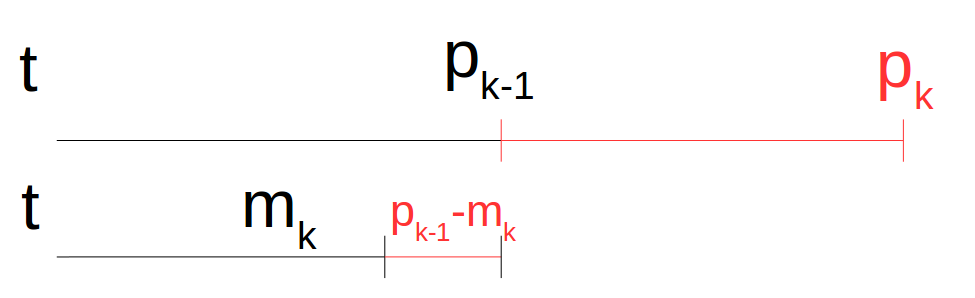
\includegraphics[width=90mm]{q6.png}
\caption{Timeline of two items processing\label{overflow}}
\end{figure}

When the benefits of parallel polishing is realised, $p_k$ can be polished at $m_k$, rather than wait the 'dead time' of $p_{k-1}-m_k$ - this figure then becomes the time saved for these two items or:
\[t_s = p_{k-1} - m_k \]
Thus, to maximise $t_s$ (and reduce the time taken to process these two items), we either maximise $p_{k-1}$ or minimise $m_k$ which is what the order in equation (16) tries to greedily achieve.
As items are introduced to the miller in series, this situation will generalise across all items, thus showing that this is the optimal order.



\maketitle{\textbf{Question 7}}

We require a spanning tree across the entire connected graph with largest weight in the graph is minimised.
One approach is using Kruskal's algorithm to greedily select minimum weight edges from a set of all edges and their weights in the graph (only adding to the spanning tree if the addition of the edge does not form a cycle) until a spanning tree is obtained.

Each choice is the local minimum edge and extrapolated out throughout the tree presents the choice of tree with minimal overall weight.

The general steps are:
\begin{lstlisting}[frame=single]
start with empty minimum spanning tree (MST)
consider edges in increasing weight order
add edge if it does not form a cycle in MST
repeat until V-1 edges are added
\end{lstlisting}

Multiple minimum spanning trees can exist in the case that there are two edges with equal weighting.However, this will not effect what the smallest weight of an edge is in the tree, as the edges are chosen based on the weight itself - the weight of the solution is independent of the 'path' taken to get to the tree.

\maketitle{\textbf{Question 8}}

Assume that Telstra base towers' 5km is unidirectional rather than radial (linear road).
Starting at Loologong and heading towards Goolagong, say that that each tower covers the last 5km stretch of road in the Loolagong direction (behind it).

The algorithm works as pseudocode follows:
\begin{lstlisting}[frame=single]
while (distance travelled < (Loologong - Goolagong)) {
  if (house in range) {
    walk 5km, then place base tower
  } else {
    while (no houses in range) {
      Proceed unit distance toward Loologong
    }
  }
}
\end{lstlisting}

To ensure all houses are covered, any time a house is encountered in the algorithm, that single house must be reached.To be greedy in the parameter of house coverage, rather than place the base station immediately when the house $h_i$ becomes in range, we continue to the fringe of the base tower range so that $h_i$ receives coverage as well as any potential houses along the way. As the range is 5km on each tower, we don't worry in between if houses within this interval are not checked. 

However, once the tower is placed the process repeats - unit of distance (choose this sensitive enough so that houses are not missed) is covered and checked if any houses are in range at that point and the above logic is reapplied until Goolagong is reached.

The Greedy aspect ensures all houses covered whilst staying within the 5km constraint of the base tower, yielding the optimal outcome (where minimal base stations are used)

\maketitle{\textbf{Question 9}}

Sequentially remove based on 2 conditions:

1. Every invitee must know at least 5 other people

2. Every invitee must not know at least 5 other people

First, check pair list and eliminate any candidates who know less than 5 people.
Recalculate pair list (as any removed on first pass through can mean remaining candidates know less people) and repeat until no further candidates can be removed based on the number of people they know only.
Now, starting from most connected (know most people), eliminate those who have less than 5 people whom they are not paired with in the list, again recalculating pair least after each pass. Stop when no further candidates can be removed.
The first step must then be repeated as the process of removing based on condition 2 has removed some from the pool. Existing candidates that survived the first pass of condition 1 must now be re-examined as their contacts may have been eliminated, reducing their pool of people they know (and hence eligibility to be invited).

Repeat these two iterative pass patterns until no candidates can be removed on a pass through the list checking both conditions consecutively - the remaining list of candidates are the maximum subset of invitees from the original list. 
(Can be implemented recursively, calling less a set \& list of less people each time)

This subset is the largest number of possible invitees as the set was built by eliminating from the whole set - i.e. it started with everyone and only reduced if any candidate fails to meet Alice's condition. Further, recalculating with each reduction ensures the 2 conditions are followed to according to contents of the current subset of candidates at all times. Hence, this means no unecessary eliminations and gives the largest number of eligible invitees in the subset.

\vspace{10mm}

\maketitle{\textbf{Question 10a)}}

This strategy fails when the pattern of white and black dots have an alternating black and white dot on each end, has one repeat after beginning and continues alternating throughout i.e.
\[BBW  \dots  BWBW  \dots  BW \]
As this strategy always connects the two dots closest together first, the end black and white dots will get merged last, resulting in unecessarily long length of wire to connect them, making the length sub-optimal. For example with this pattern:
\[WWBBWB\]

Using the given strategy, a length of 7 is reached: the middle two pairs are connected $WB$ and $BW$with the sandwiching $WB$ contributing the final distance of 5. However, if an alternate strategy of just connecting the closest matching dot from the left would give:
2 from $W$ with $B$ in $WWB$, 2 from $W$ and $B$ in $WBB$ and finally 1 from the remaining 2 $BW$ dots for a total length of 5. Clearly, the alternative approach achieved a lower length than the proposed algorithm, showing that it is not optimal in this case.
 
\maketitle{\textbf{Question 10b)}}

As we saw in part a), marrying black and white dots closest to each other first does not always yield the optimal solution - when there are stragglers with no adjacent connecting dot, the connecting wire is stretched out to the other side of the array (longer wire cost).

To even out the imbalance in wire cost, an alternate method is to be greedy on minimising wire length from left to right (one direction to the other, either works). Whenever a dot is encountered, scan remaining dots and connect it to the first available opposite colour dot.
Whilst it does not prioritise every adjacent dot to be connected, it will find a matching dot which uses the least wire for the current dot which will average out to be minimal wire as the minimum choice is taken with each step (each new dot).

To show optimal, consider a model situation between two sets of dots.
Where wire cost is given by W, dot indexes are w and b respectively:
With L representing left most dots, and L+1 being next one along the cost of connecting 2 wires can be modelled below.

Say that the greedy strategy was not correct. Rather than connecting leftmost $w_L$ to $b_L$ the optimal would go for an alternative, in this case $b_L$. Hence, the costs would be:
\[ W(w_L,b_{L+1}) + W(w_{L+1}, b_L)\] 

In the greedy algorithm's case:
\[ W(w_L,b_L) + W(w_{L+1}, b_{L+1}) \]

There are 3 possible arrangements for the dots (caps for actual dots, lowercase for distance) with differing results.
\[ W_L \quad B_L \quad W_{L+1} \quad B_{L+1} \]

When $b_{L+1} > w_{L+1}$, clearly $b_{L+1} - w_{L} > b_L - w_L$ - there is a saving in connecting L dots and L+1 dots together.

\[ W_L \quad B_L \quad W_{L+1} \quad B_{L+1} \]
Similarly, when $b_L < b_{L+1} < w_{L+1}$, $b_{L+1} - w_L > b_L - w_L$ and a saving scenario occurs for $w_{L+1} - b_L$ compared to $w_{L+1} - b_{L+1}$.

\[ W_L \quad B_L \quad W_{L+1} \quad B_{L+1} \]
Here, distances are equal.

This is a contradiction - clearly greedy solution presents distance (and hence cost savings) for 2 of 3 possible permutations of alternate dots. Hence, greedy solution must be optimal.

\vspace{5mm}

\maketitle{\textbf{Question 11}}

Assume that choosing the first task will result in completing that task and avoiding the penalty (and avoiding first penalty will allow next penalty to be avoided/minimum if next choice is optimal, etc)
Choose greedily - Sort tasks in descending order of penalty with concession.
With each new task to choose, compute $\Sigma p_{i}$ from $n = i+1 to n_{finalTask}$  where $p_i$ is penalty of current task. Compare the two values, and if the sum is greater then pick the greatest penalty task within the remaining task-list to do first. Repeat this until all compatible tasks are chosen.

Since all tasks take the same amount of time doing highest penalty value tasks first will minimise the penalty with each new task choice and also consider when a build up of avoiding earlier small penalty tasks will outweigh the bonus of avoiding a singular task with large penalty.



\maketitle{\textbf{Question 12}}

To choose, use the foresight of knowing which books you will need to greedily choose the next 10 books to exchange. Consider the sequence of books required as an array of B = $B_i $ for $i = 0 \dots n_{books}$.

First, take loans on $B_1 \dots B_10$, add them to a set of unique borrowed books borrowedBooks and pop off and delete books as required $B[i]$ from B if borrowedBooks.contains($B[i]$) is true. Repeat pop off until a new unique book (say, $B_{11}$) occurs in B which is not in borrowedBooks (borrowedBook.contains($B_{11}$) is false).

At this point, make the greedy choice and exchange all current books (empty the borrwedBooks set of currently borrowed books and note count of trips so far) and scan across B from the index that $B_11$ occurred. Starting with $B_{ 11 }$, add every unique book encountered until borrowedBooks has 10 elements ($n_{borrowedBooks}$ = 10).Repeat the previous process as books are 'checked' and popped off until again, a new book $B_k$ is encountered and another exchange is absolutely necessary. The number of exchanges that occur when the end of array B is reached will then be the minimum number of trips.

This strategy minimises trips to exchange as it projects the inventory of books to stretch as far into future books needed as permitted by the size of inventory (10). Bearing in mind required books in B can repeat, scanning for unique set and checking if they are available (borrowedBooks.contains) will choose the maximum possible subset of B satisfied by the current borrowedBooks array at any time.

\maketitle{\textbf{Question 13}}

Consider stalls $1\dots n$:
For all stalls, mark start and finish points (in stall number) of potential planks requiring a plank and use as coordinates.
e.g. (0,0), (3,3), (5,8) means that stall 0, 3 require a plank and have no adjacent stalls to cover as well, whilst stalls 5-8 require coverage.
Repeat this coordinate transformation for all stalls requiring coverage from the 0th stall and consider the 'distance' in stall number from each other. This is computable by $d_{internal} = n_{finish} - n_{start}$.
Sort this list of distances and related coordinates in descending order as largest internal distance indicates largest run of consecutive stalls.
Hence, initially cover stalls in this order until all boards are covered/11 boards are used up.
In some cases, this will not be optimal (not all required stalls are consecutive).
In order to extend the algorithm to use the same boards to close small gaps to cover more required stalls - Further, compute the distance BETWEEN coordinates, i.e
\[ d_{between} = n_{istart} - n_{(i-1)finish} \]

Now, resorting the list of priorities to reflect $d_{between}$, pick the appropriate stall to extend the board and increase the internal distance within the stall (maximise consecutive required stalls covered by boards).

Repeat this until iterations no longer make any changes in order of boards to have the state of the stall array/other data structure cover all required stalls.


\maketitle{\textbf{Question 14}}

If B's string contains a subarray of the contents of A, then the letters in B will:

a) also be in A
b) occur A in the same order they do in B

Determining whether this is true can be found as follows:

First, save the original number of elements in B $n_{original}$ (later used to stop algorithm).
To ensure this, first scan through sequence of letters (say, an array) in A and check if a match is found ($A[i]$ equals $B[n]$ - where $n = 0$; first letter in potential subsequence B).

Here, use array B to keep track of when matches are found.
If a match is found for $A[k]$, delete all $A[j]$ for $j = 0 \dots k$ (deleting marks these letters as having been considered) and delete $B[n]$ to mark that it has been found in the array.

Check remaining number of elements - $n_{length of B}$ and update checked original numbers  ($n_{original} += -1$) to signify the first element of B has been checked. If B is empty, then all letters in B have been found in A in the correct order (satisfying conditions a) and b)) and hence the algorithm returns true. Otherwise continue.

Repeat the above process for the remaining $n = 1 \dots n_{length of B}$, stopping when A has been scanned for and $n_{original}$ reached or the B isEmpty check (described above) above determines that B is indeed a subarray of A.
If the algorithm has exhausted all elements and $B$ remains non-empty, then not all elements in $B$ have been found in the correct order (deleting $A[j]$ for $j = 0 \dots k$ above ensures out of order letters are not checked) - B does not contain a sub-array of A.


%$n_{eltsA} = n_{eltsB} = n$. This will involve iterating over A and deleting based on a false B.contains($A_i$) return value.
%Now, check if the contents match in the right order. This can be described iteratively by the below pseudocode in $O(n_{eltsA}n_{eltsB})$ time.
%
%for (i = 0; i < A.length; i++)
%    order = false
%    j = 0; k = i;
%    for (j =0; j < B.length; j++)
%      k = i + j
%      if (B[j] = A[k])
%        order = true
%     else
%        order = false

%If the above algorithm returns true, then B contains a subArray of A.

%The deletion step so that the number of elements is the same can be done within the above pseudocode by checking if A contains B[j] on each iteration and deleting if so.

\end{document}



